\chapter{Primes, GCD, and and the intrigue of Cryptography}

\begin{figure}[ht]       
\centerline{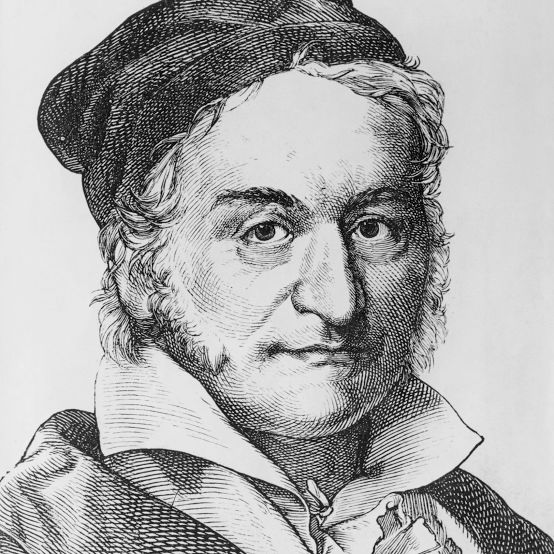
\includegraphics[width=1.0in]{images/gauss.jpeg}}
\caption*{\small ``The primes are the jewels in the crown.'' -- Carl Friedrich Gauss}
\end{figure}

\begin{figure}[ht]
\centerline{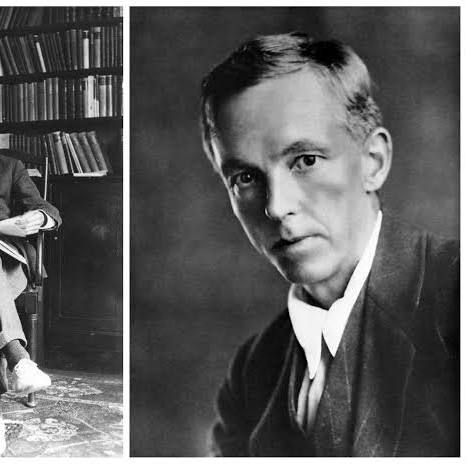
\includegraphics[width=1.0in]{images/Hardy.jpeg}}
\caption*{\small ``A mathematician, like a painter or a poet, is a maker of patterns. If his patterns are more permanent than theirs, it is because they are made with ideas. And the primes are the most eternal patterns of all.'' -- G. H. Hardy}
\end{figure}

\begin{figure}[ht]
\centerline{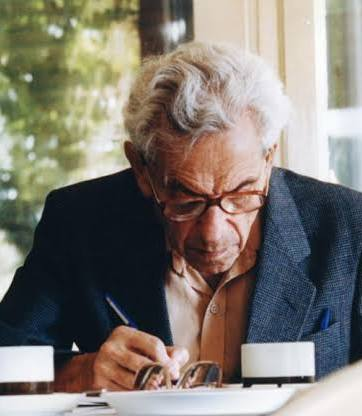
\includegraphics[width=1.0in]{images/Erdoss.jpeg}}
\caption*{\small ``God may not play dice with the universe, but something strange is going on with the prime numbers.'' --  Paul Erd\H{o}s}
\end{figure}

The theory of prime numbers and their properties forms the foundation of number theory.  At first sight, the study of primes may seem like a purely mathematical pursuit. 
Yet today prime numbers play a crucial role in modern life, because they underpin  cryptographic systems that secure communication over the internet. 

In this chapter we introduce the basic ideas of primes and factorisation, 
methods for computing greatest common divisors, some crucial algorithms and theorems about primes, 
and finally explain how these notions are used in public-key cryptography, especially the \href{https://en.wikipedia.org/wiki/RSA\_cryptosystem}{RSA cryptosystem}.

\section{Primes}

We have informally discussed primes several times in these notes. We give a formal definition here
\begin{definition}
A \emph{prime number} is an integer $p > 1$ whose only positive divisors are $1$ and $p$ itself.
\end{definition}

Numbers greater than 1 that are not prime are called \emph{composite}.  
$2,3,5,7,11$ are some examples of primes, while $12=3 \times 4$ is composite.  In what follows, we develop some properties of prime numbers.

\subsection{There are infinitely many primes}

In Theorem \ref{thm:infiniteprimes} we proved there are infinitely many primes. We repeat the theorem here for the sake of completeness.

\begin{theorem}[Euclid]
There are infinitely many prime numbers.
\end{theorem}
\begin{proof}
Suppose there are only finitely many: $p_1,\dots,p_k$. 
Consider $N=p_1\cdot p_2\cdots p_k+1$. 
No $p_i$ divides $N$, since each leaves remainder $1$. 
Thus $N$ is prime or divisible by a new prime, contradicting the assumption\footnote{Assume you have a finite list of primes. Multiply them together and add 1. Either that number is prime — or you just found a new factor. Either way, you’re wrong. Welcome to mathematics!}. 
\end{proof}
\vspace{2mm}

\subsection{Unique prime factorisation}

The  \emph{Unique Prime Factorisation theorem}  (Theorem \ref{thm:primefactor}) establishes that primes are the ``atoms'' of arithmetic: every integer factors into primes, and no further. We again repeat it here for completeness.
\begin{theorem}[Fundamental Theorem of Arithmetic]
Every integer $n>1$ can be written as a product of primes. 
This factorisation is unique up to the order of the factors.
\end{theorem}
\begin{proof}
\emph{Existence:} If $n$ is prime, we are done. Otherwise, assume that the claim is true for all $m$ such that $2 \leq m < n$. Let  $n=ab$ with $a,b<n$. By the induction hypothesis, each of $a$ and $b$ has a prime factorisation, hence so does $n$.

\emph{Uniqueness:} Suppose
\[
n = p_1p_2\cdots p_k = q_1q_2\cdots q_m
\]
with all $p_i, q_j$ prime. Then $p_1$ divides the right side, hence some $q_j$. But since $q_j$ is prime, $p_1=q_j$. Cancelling, we continue inductively to conclude that the multisets $\{p_i\}$ and $\{q_j\}$ are identical.
\end{proof}

\subsection{The Sieve of Eratosthenes}

One of the oldest known algorithms for finding prime numbers is due to 
\emph{Eratosthenes of Cyrene} (around 200 BCE). 
The method, called the \href{https://en.wikipedia.org/wiki/Sieve\_of\_Eratosthenes}{Sieve of Eratosthenes}, systematically eliminates 
composite numbers from a list, leaving only primes.

\begin{quote}
Sift the Two's and Sift the Three's: \\
The Sieve of Eratosthenes. \\
When the multiples sublime, \\
The numbers that remain are Prime. \\

\hspace{1.0in}	-- Anonymous
\end{quote}

\subsubsection*{The Algorithm}
To find all primes up to a given number $N$:

\begin{enumerate}
\item Write down the list of integers $2,3,4,\dots,N$.
\item Start with the first number $p=2$. It is prime.
\item Cross out all multiples of $p$ greater than $p$ itself in the list.
\item Find the next uncrossed number. This is the next prime. Set $p$ to this number and repeat Step 3.
\item Continue until $p^2 > N$. All remaining uncrossed numbers are prime.
\end{enumerate}

\begin{example}{Primes up to 30}

\begin{figure}[h]
\centering
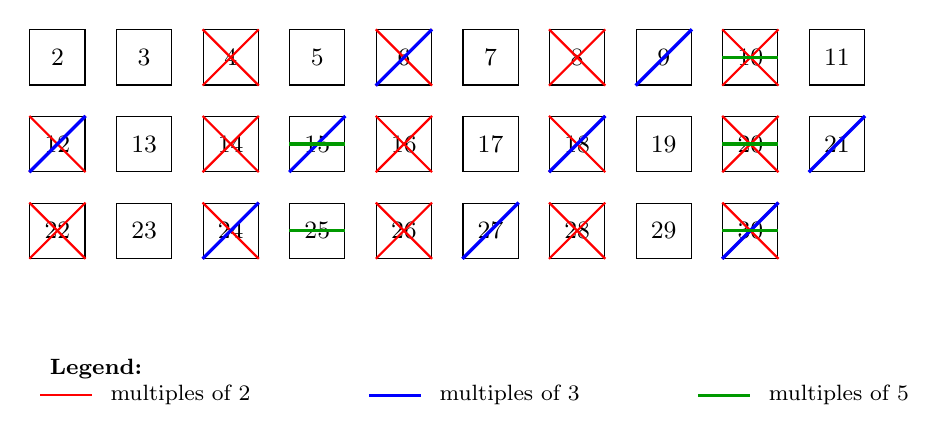
\begin{tikzpicture}[>=stealth, x=1.1cm, y=1.1cm]
  % Style for number boxes
  \tikzstyle{num}=[draw, minimum width=7mm, minimum height=7mm, align=center]

  % Place numbers 2..30 in a 3x10 grid (10 per row)
  \foreach \n [count=\k from 1] in {2,...,30}{
    \pgfmathtruncatemacro{\col}{mod(\k-1,10)}
    \pgfmathtruncatemacro{\row}{floor((\k-1)/10)}
    \node[num] (N\n) at (\col,-\row) {\small \n};
  }

  % Cross out composites:
  % Multiples of 2 (>=4): red X
  \foreach \m in {4,6,8,10,12,14,16,18,20,22,24,26,28,30}{
    \draw[red, thick] (N\m.south west) -- (N\m.north east);
    \draw[red, thick] (N\m.south east) -- (N\m.north west);
  }

  % Multiples of 3 (>=6): blue diagonal (overlay)
  \foreach \m in {6,9,12,15,18,21,24,27,30}{
    \draw[blue, very thick] (N\m.south west) -- (N\m.north east);
  }

  % Multiples of 5 (>=10): green horizontal (overlay)
  \foreach \m in {10,15,20,25,30}{
    \draw[green!60!black, very thick] (N\m.west) -- (N\m.east);
  }

  % Legend
  \node[anchor=west] at (-0.2, -3.6) {\footnotesize \textbf{Legend:}};
  \draw[red, thick] (-0.2,-3.9) -- +(0.6,0);
  \node[anchor=west] at (0.5,-3.9) {\footnotesize multiples of 2};
  \draw[blue, very thick] (3.6,-3.9) -- +(0.6,0);
  \node[anchor=west] at (4.3,-3.9) {\footnotesize multiples of 3};
  \draw[green!60!black, very thick] (7.4,-3.9) -- +(0.6,0);
  \node[anchor=west] at (8.1,-3.9) {\footnotesize multiples of 5};
\end{tikzpicture}
\caption{Sieve of Eratosthenes up to 30. Uncrossed boxes are primes.}
\label{fig:sieve}
\end{figure}

Start with the numbers $2$ to $30$ (see Figure \ref{fig:sieve}).

\begin{itemize}
\item $2$ is prime. Cross out $4,6,8,\dots,30$.
\item Next uncrossed is $3$. Cross out $6,9,12,\dots,30$.
\item Next uncrossed is $5$. Cross out $10,15,20,25,30$.
\item Next uncrossed is $7$. Since $7^2=49>30$, we stop.
\end{itemize}

The remaining numbers are $2,3,5,7,11,13,17,19,23,29$, exactly the primes $\leq 30$.
\end{example}
\subsection*{Remarks}
\begin{itemize}
\item The sieve is simple and efficient for generating primes up to a moderately large bound.
\item It takes  $O(N \log \log N)$ steps for large $N$, making it far faster than testing each number individually for divisors.
\item This method, though ancient, is still used sometimes\footnote{Unfortunately, this algorithm is too inefficient in practice. The problem of primality testing -- how to test whether a given integer is a prime -- has been open  at least since the times of Euclid and Eratosthenes. The first ``efficient'' solution for the problem was the \href{https://en.wikipedia.org/wiki/AKS_primality_test}{AKS algorithm from IIT Kanpur} in 2002. In practice, an even faster \href{https://en.wikipedia.org/wiki/Miller–Rabin_primality_test}{Miller-Rabin test} is used, but it uses probabilistic coin tosses as a primitive, and can give a wrong answer with a very small probability. We will study some of these methods later in these otes}.
\end{itemize}

\begin{exercise}
Find all primes between 2 and 100 using the Sieve of Eratosthenes.
\end{exercise}

\subsection{The Prime Number Theorem}

The distribution of primes among the natural numbers is highly irregular: 
sometimes primes cluster close together, other times they are far apart. 
A natural question, posed already by \href{https://en.wikipedia.org/wiki/Carl\_Friedrich\_Gauss}{Gauss} and \href{https://en.wikipedia.org/wiki/Adrien-Marie\_Legendre}{Legendre} around the year 1800 when he was a teenager\footnote{Historians like to quip: ``Even at 15, Gauss preferred to keep his prime secrets private.''}, is:
\emph{How many primes are there up to a large number $n$?}

\begin{theorem}[\href{https://en.wikipedia.org/wiki/Prime\_number\_theorem}{Prime Number Theorem}]
\label{thm:primenumber}
Let $\pi(n)$ denote the number of primes $\leq n$. Then
\[
\pi(n) \sim \frac{n}{\ln n}, \quad \text{as } n \to \infty,
\]
meaning that
\[
\lim_{n\to\infty} \frac{\pi(n)}{n/\ln n} = 1.
\]
\end{theorem}

\begin{figure}[h]
\centering
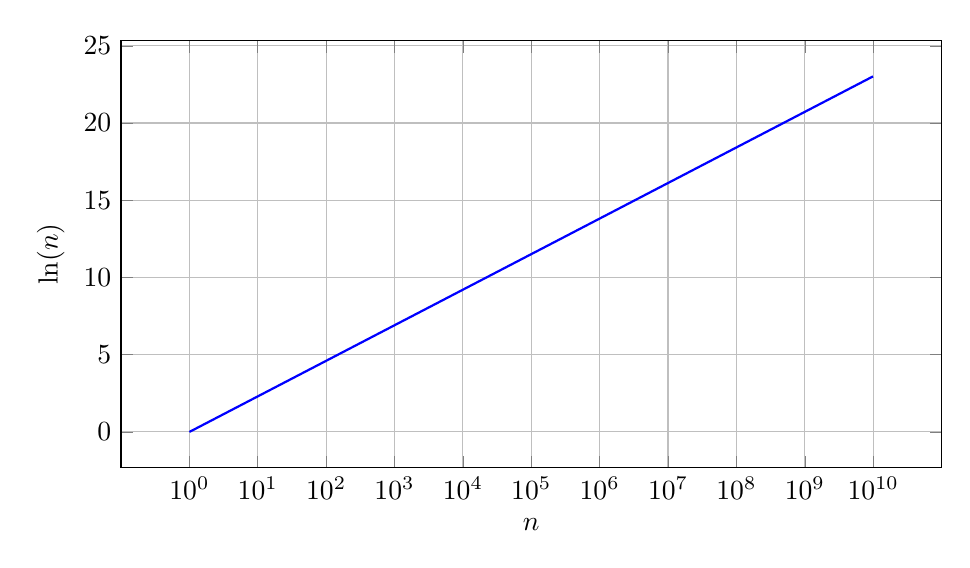
\begin{tikzpicture}
\begin{semilogxaxis}[     % log scale on x-axis
    xlabel={$n$},
    ylabel={$\ln(n)$},
    width=12cm, height=7cm,
    log basis x=10,
    xtick={1,10,100,1000,10000,100000,1000000,10000000,100000000,1000000000,10000000000},
    xticklabels={$10^0$,$10^1$,$10^2$,$10^3$,$10^4$,$10^5$,$10^6$,$10^7$,$10^8$,$10^9$,$10^{10}$},
    ytick={0,5,10,15,20,25},
    grid=both
]
\addplot[domain=1:1e10, samples=500, thick, blue] {ln(x)};
\end{semilogxaxis}
\end{tikzpicture}
\caption{The natural logarithm $\ln(n)$ grows very slowly, even as $n$ reaches $10^{10}$.}
\label{fig:lnn}
\end{figure}


In words: the density of primes around $n$ is roughly $\tfrac{1}{\ln n}$.  The \href{https://en.wikipedia.org/wiki/Natural\_logarithm}{natural logarithm function} $\ln n$ is a rather slowly growing function. It can be intuitively understood as a way of answering the question: ``How much time does it take to grow from 1 to $n$, assuming continuous growth at a fixed rate?". See Figure \ref{fig:lnn} for a plot. We will revisit the natural logarithm function later in these notes. So, primes are not very sparse at all\footnote{Carl Friedrich Gauss (1792–93), as a teenager, investigated prime tables and conjectured the approximation $\pi(n) \approx \operatorname{Li}(n)$, where $\operatorname{Li}(n) = \int_2^n \tfrac{dt}{\ln t}$ is the logarithmic integral.  He recorded this insight in his diary, long before publishing it. Adrien-Marie Legendre independently proposed the formula $\pi(n)\approx \tfrac{n}{\ln n - 1.08366}$ in 1798. The theorem was finally proved independently in 1896 by \href{https://en.wikipedia.org/wiki/Jacques\_Hadamard}{Jacques Hadamard}  and \href{https://en.wikipedia.org/wiki/Charles\_Jean\_de\_la\_Vall\%C3\%A9e\_Poussin}{Charles Jean de la Vall\'ee Poussin}, using complex analysis and properties of the Riemann zeta function.   Their proof showed how deep connections between prime numbers and complex analysis truly are. Interested students will have to wait for a few later course in mathematics to study the proofs}.
For example, around $n=10^6$, about one in every $14$ numbers is prime.

The proof of the prime number theorem is unfortunately out of the scope of these notes. Interested readers will have to follow up QRMT with some courses on calculus, analysis and algebra for the proof to be accessible.

\begin{exercise}
Use a calculator to stimate the number of primes between $10^6$ and $10^7$ using the prime number theorem.
\end{exercise}


\subsection{Fermat’s Little Theorem}

Prime numbers have remarkable properties in modular arithmetic. 
One of the most beautiful and useful is a result discovered by \href{https://en.wikipedia.org/wiki/Pierre\_de\_Fermat}{Pierre de Fermat} in 1640, 
long before the modern development of number theory. 
It shows that when we raise a number to a large power, the remainder upon division by a prime 
behaves in a very simple way.

Fermat wrote that if $p$ is a prime and $a$ is not divisible by $p$, then
$a^{p-1} \equiv 1 \pmod p$. 
He gave no proof, and the first rigorous demonstrations came later from \href{https://en.wikipedia.org/wiki/Leonhard\_Euler}{Leonhard Euler} and others.

This theorem is central in number theory. 
It lies behind efficient algorithms for primality testing, 
and it forms one of the key mathematical tools used in public-key cryptography.
Before proving it, let us state it precisely.
\begin{theorem}[Fermat’s Little Theorem]
\label{thm:fermat}
If $p$ is prime and $p\nmid a$, then
\[
a^{p-1}\equiv 1 \pmod p.
\]
\end{theorem}
\begin{proof}
Multiplication by $a$ permutes the set $\{1,2,\dots,p-1\}$ modulo $p$ (why?)
Thus
\[
a\cdot 2a\cdots (p-1)a \equiv 1\cdot 2\cdot \cdots (p-1) \pmod p.
\]
This gives $a^{p-1}(p-1)!\equiv (p-1)! \pmod p$. Since $(p-1)!$ is not divisible by $p$, we may cancel to obtain $a^{p-1}\equiv 1 \pmod p$.
\end{proof}

\begin{exercise}
Argue that multiplication by $a$  permutes the set $\{1,2,\dots,p-1\}$ modulo $p$. That is, the operation is injective.
\end{exercise}


The Fermat's little theorem  can be used for primality testing as follows:

\subsubsection*{Fermat Primality Test Algorithm}

\begin{enumerate}
\item Given an integer \( n > 2 \), choose a random integer \( a \) where \( 1 < a < n-1 \) and \( \gcd(a, n) = 1 \).
\item Compute \( a^{n-1} \bmod n \).
\item If 
\[
a^{n-1} \not\equiv 1 \pmod{n},
\]
then \( n \) is definitely composite.
\item If 
\[
a^{n-1} \equiv 1 \pmod{n}
\]
holds for several randomly chosen values of \( a \), then \( n \) is probably prime.
\end{enumerate}

\subsubsection*{Limitations}
\begin{itemize}
\item The test is \emph{probabilistic}, not deterministic.
\item Certain composite numbers, known as \textit{Fermat pseudoprimes}, can satisfy the congruence for some bases \( a \), causing false positives.
\item To reduce error probability, test multiple values of \( a \) independently.
\end{itemize}

\begin{example}
For \( n = 11 \):
\[
2^{10} \equiv 1 \pmod{11}, \quad 3^{10} \equiv 1 \pmod{11},
\]
so 11 is probably prime.

For a composite number \( n = 15 \):
\[
2^{14} \not\equiv 1 \pmod{15},
\]
so 15 is composite.
\end{example}


\section{The Greatest Common Divisor}

\begin{figure}[ht]
\centerline{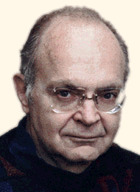
\includegraphics[width=1.0in]{images/don.jpg}}
\caption*{\small ``The Euclidean algorithm is one of the oldest nontrivial algorithms that has survived to the present day. It can be considered the first efficient algorithm ever devised.'' -- Donald Knuth}
\end{figure}

%\begin{figure}[ht]       
%\centerline{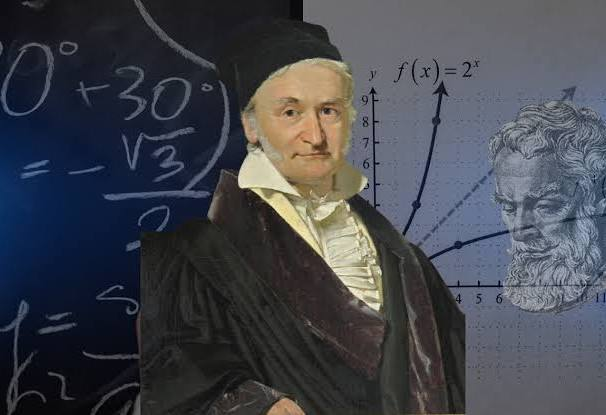
\includegraphics[width=1.0in]{images/gauss2.jpg}}
%\caption*{\small ``The algorithm of Euclid is the finest jewel in the crown of elementary number theory.'' -- Carl Friedrich Gauss}
%\end{figure}


When working with integers, one of the most natural questions is: given two numbers, 
what is the largest number that divides them both? For example, for $18$ and $24$ the answer is $6$, 
since $6$ is the largest integer that divides both without remainder. 
This simple idea is called the \emph{greatest common divisor}, or \emph{gcd} for short.

The gcd plays a central role in number theory. It captures the notion of 
the ``common part’’ of two numbers, and it is fundamental for simplifying fractions, 
solving equations in integers, and developing modular arithmetic. 
As we will see, the efficient algorithm to compute gcds, due to Euclid, 
is one of the oldest and most beautiful algorithms in all of mathematics.

\begin{definition}
The \emph{greatest common divisor} $\gcd(a,b)$ of two integers $a,b$ is the largest integer that divides both.
\end{definition}

\begin{example}
\[
\gcd(18,24)=6, \qquad \gcd(13,27)=1.
\]
\end{example}


\subsection{Euclid’s Algorithm}
Euclid, over 2000 years ago, discovered a remarkably efficient method, $Euclid\_gcd$, for computing $\gcd(a,b)$, $a > 0, b \geq 0$:
\begin{eqnarray*}
\begin{array}{ll}
Euclid\_gcd(a,b) = a & \mbox{if $b=0$} \\
Euclid\_gcd(a,b) = Euclid\_gcd(b,\, a \bmod b) & \mbox{otherwise}
\end{array}
\label{algo:Egcd}
\end{eqnarray*}
Repeating this step until the remainder is $0$ yields the gcd.

\begin{example}
To compute $\gcd(252,105)$:
\[
252=105\cdot2+42, \quad Euclid\_gcd(252,105)=Euclid\_gcd(105,42),
\]
\[
105=42\cdot2+21, \quad Euclid\_gcd(105,42)=Eucid\_gcd(42,21),
\]
\[
42=21\cdot2+0 \quad\Rightarrow\quad Euclid\_gcd(21,0) =21.
\]
\end{example}


\subsubsection{Correctness of Euclid's GCD algorithm}

To prove the correctness of Euclid's algorithm, we first require the following result which was
proved by Euclid. \newline
{\bf Claim:} If $a = qb + r$, $0 < r < b$, then $gcd(a,b) = gcd(b,r)$ \newline
\begin{proof}
If $d = gcd(a,b)$ then $d \mid a$ ($d$ divides $a$) and $d \mid b$ which, in turn, implies that
$d \mid (a - qb)$, or $d \mid r$. Thus $d$ is a common divisor of $b$ and $r$.
If $c$ is any common divisor of $b$ and $r$, then $c \mid (qb + r)$ which implies
that $c \mid a$. Thus $c$ is a common divisor of $a$ and $b$. Since $d$ is the largest
divisor of both $a$ and $b$, it follows that $c \leq d$.
It now follows from definition that $d = gcd(b,r)$.
\end{proof}

We can then prove the correctness of $Euclid\_gcd$ using the principle of mathematical induction.

\begin{theorem}
 For all $b \geq 0$, for all $a > 0$, $Euclid\_gcd(a,b)$ computes $\gcd(a,b)$, the largest common divisor of $a$ and $b$.
 \end{theorem}

\begin{proof}
\begin{description}
\item[Basis.] $b = 0$. If $b = 0$ then for all $a > 0$, 
      $Euclid\_gcd(a,b) = a = gcd(a,b)$.
\item[Induction hypothesis.] For all $b \leq k$ such that $0 \leq b$, for all $a > 0$,
         $Euclid\_gcd(a,b) = gcd(a,b)$.
\item[Induction step.] Consider $b = k+1$,  $a > 0$. 
         \[
         \begin{array}{llll}
         Euclid\_gcd(a,b) & = & Euclid\_gcd(b,a\;mod\;b) \\
                & = & gcd(b,a\;mod\;b) & \mbox{by the inductive hypothesis} \\
                & = & gcd(a,b) & \mbox{by the Claim above}
         \end{array}
         \]
\end{description}
\end{proof}


\begin{definition}
Two positive integers are  \emph{relatively prime} if their gcd is 1, i.e.,  they have no non-trivial factors in common.
\end{definition}

\subsection{The Extended Euclidean Algorithm}



Euclid’s algorithm is remarkable because it quickly computes the gcd of two numbers. 
But sometimes we need more than just the gcd: we want to write the gcd 
as a sum of multiples of the two numbers themselves\footnote{Euclid tells us what the gcd is; the extended Euclid tells us how to make it.}.

For example, for $a=30$ and $b=12$, not only is $\gcd(30,12)=6$, but also
\[
6 = 30 \times (-1) + 12 \times 3.
\]

In other words, the gcd can be expressed as a whole-number combination of $a$ and $b$.  This means we can “build” the gcd by taking suitable multiples of $30$ and $12$.
This fact is called \href{https://en.wikipedia.org/wiki/B\%C3\%A9zout\%27s_identity}{B\'ezout's identity}. 

The \emph{Extended Euclidean Algorithm} is just a way to find these multipliers
at the same time as we compute the gcd. 

\paragraph{How it works (idea).}
We start the same way as in Euclid’s algorithm:
\[
a = q_1 b + r_1, \quad b = q_2 r_1 + r_2, \quad \dots
\]
until we reach a remainder $0$.  
While we do this, we also keep track of how each remainder is made from $a$ and $b$.  
At the end, the last nonzero remainder is the gcd, and the numbers in front of $a$ and $b$ 
give us the multipliers we want.

\begin{figure}[ht]
\centerline{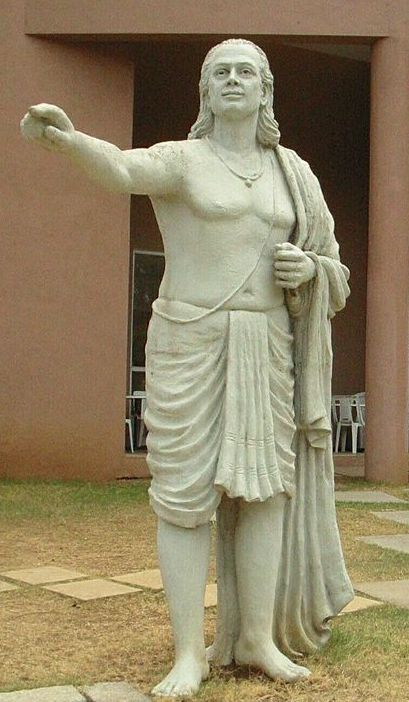
\includegraphics[width=1.0in]{images/Aryabhata_IUCAA.jpg}}
\caption*{\={A}ryabha\d{t}a's statue in the Inter-University Centre for Astronomy and Astrophysics (IUCAA) at Pune}
\end{figure}

\begin{example}
Let’s find the gcd of $26$ and $7$, and also write it as a combination of $26$ and $7$.

\[
26 = 3 \times 7 + 5, \quad
7 = 1 \times 5 + 2, \quad
5 = 2 \times 2 + 1, \quad
2 = 2 \times 1 + 0.
\]

So $\gcd(26,7)=1$.  

Now work backwards:
\[
1 = 5 - 2 \times 2,
\]
\[
1 = 5 - 2 \times (7 - 1 \times 5) = 3 \times 5 - 2 \times 7,
\]
\[
1 = 3 \times (26 - 3 \times 7) - 2 \times 7 = 3 \times 26 - 11 \times 7.
\]

So we have
\[
1 = 3 \times 26 + (-11) \times 7.
\]

This shows that $-11$ is a multiplier for $7$ that makes $7 \times (-11) \equiv 1 \pmod{26}$.  
In other words, $7$ has an inverse modulo $26$, and it is $15$ (since $-11 \equiv 15 \pmod{26}$) \footnote{We had discussed this earlier in Theorem \ref{thm:diaphontine}. The origins of this algorithm can be traced back to  \={A}ryabha\d{t}a ($5^{th}$ c), Jayadeva (c. $10^{th}$–$11^{th}$ c.) and later Bh\'{a}skara II ($12^{th}$ c.). Bh\'{a}skara in the L\={\i}l\={a}vat\={\i} and B\={\i}jaga\d{n}ita gives worked examples of solving linear Diophantine equations with what is recognizably the extended Euclid method.}.  
\end{example}

The steps of the general algorithm can then be given as:

\paragraph{General Algorithm (Extended Euclid).}

\label{algo:extended-Euclid}
Given two integers $a$ and $b$:

\begin{enumerate}
\item If $b=0$, then $\gcd(a,0)=a$ and we return $(x,y)=(1,0)$.
\item Otherwise, divide $a$ by $b$: 
\[
a = q b + r, \quad 0 \leq r < b.
\]
\item Inductively apply the algorithm to $(b,r)$ to get
\[
\gcd(b,r) = xb + yr.
\]
\item Substitute $r=a - qb$ to express the gcd in terms of $a$ and $b$:
\[
\gcd(a,b) = y a + (x - qy)b.
\]
\item Return $(x',y')=(y,\,x-qy)$.
\end{enumerate}

At the end, we obtain integers $x,y$ such that
\[
ax + by = \gcd(a,b).
\]

\begin{exercise}
(Bh\'{a}skara I, c. 600) ``Tell me at once, O mathematician, that number which leaves unity as remainder when divided by any of the numbers from 2 to 6 but is exactly divisible by 7." [Ans : 301]
\end{exercise}

\begin{exercise}
(Mah\={a}v\={\i}ra, c. 850) ``Five heaps of fruits added with two fruits were divided equally between nine travellers; six heaps added with four fruits were divided amongst eight; four heaps increased by one fruit were divided amongst seven. Tell the number of fruits in each heap.” [(Least) Ans : 194]
\end{exercise}

\paragraph{Why this matters.}
The extended Euclidean algorithm is very useful:
\begin{itemize}
\item It gives the gcd of two numbers.  
\item It shows how to write the gcd using those two numbers.  
\item If the gcd is $1$, it also finds a modular inverse, which is essential in cryptography.  
\end{itemize}

But how many steps does the Euclidean algorithm take? Is it slow or fast? Amazingly, the answer lies in the famous \href{https://en.wikipedia.org/wiki/Fibonacci_sequence}{Fibonacci sequence}\footnote{Though named after \href{https://en.wikipedia.org/wiki/Fibonacci}{Fibonacci}, also referred to as the {\em Leonardo of Pisa}, the sequence was known to ancient Indian mathematicians like \href{https://en.wikipedia.org/wiki/Pingala}{Pingala}, \href{https://en.wikipedia.org/wiki/Bharata\_(sage)}{Bharata muni}, \href{https://en.wikipedia.org/wiki/Virahanka}{Virahanka}, \href{https://en.wikipedia.org/wiki/Hemachandra}{Gopala and Hemachandra}.} defined as:
\[
\begin{array}{l}
F_0 = 0 \\
F_1 = 1 \\
F_k = F_{k-1} + F_{k-2}, \mbox{ for } i \geq 2
\end{array}
\]


The following theorem establishes the worst-case run rime of the Euclidean algorithm:

\begin{theorem}
If $a > b \geq 1$ and the invocation $Euclid\_gcd(a, b)$ performs $k \geq 1$ repeated calls, then $a \geq F_{k+2}$ and
$b \geq F_{k+1}$.
\end{theorem}

\begin{exercise}
Prove the above theorem using the principle of mathematical induction.
\end{exercise}

The following result immediately follows:
\begin{theorem}[Lam\'e's theorem]
For any integer $k \geq 1$, if $a > b \geq 1$ and $b < F_{k+1}$, then  $Euclid\_gcd(a, b)$ makes fewer than
$k$ repeated calls.
\end{theorem}

It is well known that $F_k \leq \phi^{k-1}$ for all $k > 0$, where $\phi = \frac{1+\sqrt{5}}{2}$ is the \href{https://en.wikipedia.org/wiki/Golden_ratio}{golden ratio}. 

\begin{exercise}
\begin{enumerate}
\item Prove that $F_k \leq \phi^{k-1}$ for all $k > 0$ using the principle of mathematical induction.
\item Argue that if  $b < F_{k+1} \leq \phi^k$, then the number of steps required will be approximately $\log{b}$, which is rather small. So, the algorithm is very efficient.
\end{enumerate}
\end{exercise}

\section{Chinese Remainder Theorem}


The Chinese Remainder Theorem (CRT) is one of the most beautiful and useful results in number theory. 
It says that if we know the remainder of a number when divided by several pairwise coprime moduli, 
then we can uniquely determine the number modulo the product of those moduli.

In other words, instead of working with a single large modulus, we can break a problem into 
several smaller ones, solve them separately, and then combine the answers back together. 
This is extremely powerful in computations, because working modulo small numbers is easier.

\medskip
\noindent
The theorem was discovered in ancient China, and first appeared in the work of 
Sun Tzu around the 3rd century AD, who posed problems like:
\emph{``Find a number which leaves remainder 2 when divided by 3, remainder 3 when divided by 5, and remainder 2 when divided by 7.''}  
The answer is unique modulo $3\cdot 5 \cdot 7 = 105$.

\medskip
\noindent
The CRT has many applications:
\begin{itemize}
\item Efficient computation in modular arithmetic (e.g. fast exponentiation).
\item Cryptography, especially RSA, where it is used to speed up decryption.
\item Error correction in coding theory.
\end{itemize}
Thus, the CRT is not only a striking piece of mathematics but also a practical tool.

\begin{example}{An example (\href{https://en.wikipedia.org/wiki/Sunzi_Suanjing}{Sun Tzu}, 3rd century AD).} \\

 ``There are certain things whose number is unknown. If we count them by threes, we have two left over; by fives, we have three left over; and by sevens, two are left over. How many things are there?” 


Suppose we want to find a number $N$ such that
\[
N \equiv 2 \pmod{3}, \quad 
N \equiv 3 \pmod{5}, \quad 
N \equiv 2 \pmod{7}.
\]

\noindent
Step 1. The moduli $3,5,7$ are pairwise coprime, so the CRT applies.  
The product is $M = 3 \cdot 5 \cdot 7 = 105$.

\smallskip
\noindent
Step 2. For each congruence, compute
\[
M_1 = \frac{M}{3} = 35, \quad 
M_2 = \frac{M}{5} = 21, \quad 
M_3 = \frac{M}{7} = 15.
\]

\smallskip
\noindent
Step 3. Find numbers $y_i$ such that
\[
M_1 y_1 \equiv 1 \pmod{3}, \quad 
M_2 y_2 \equiv 1 \pmod{5}, \quad 
M_3 y_3 \equiv 1 \pmod{7}.
\]

\begin{itemize}
\item $35 \equiv 2 \pmod{3}$, and $2\cdot 2 \equiv 1 \pmod{3} \implies y_1=2$.
\item $21 \equiv 1 \pmod{5}$, so $y_2=1$ works.
\item $15 \equiv 1 \pmod{7}$, so $y_3=1$ works.
\end{itemize}

\smallskip
\noindent
Step 4. Combine everything:
\[
N \equiv a_1 M_1 y_1 + a_2 M_2 y_2 + a_3 M_3 y_3 \pmod{M},
\]
where $(a_1,a_2,a_3)=(2,3,2)$.

\[
N \equiv 2 \cdot 35 \cdot 2 + 3 \cdot 21 \cdot 1 + 2 \cdot 15 \cdot 1 \pmod{105}.
\]

\[
N \equiv 140 + 63 + 30 = 233 \pmod{105}.
\]

\noindent
Step 5. Reduce: $233 \equiv 23 \pmod{105}$.

\medskip
\noindent
Therefore, the solution is 
\[
N \equiv 23 \pmod{105}.
\]

\smallskip
\noindent
Indeed, $23 \equiv 2 \pmod{3}$, $23 \equiv 3 \pmod{5}$, and $23 \equiv 2 \pmod{7}$.
\end{example}

\begin{theorem}[Chinese Remainder Theorem]
\label{thm:chinese}
Let $n_1,\dots,n_k$ be pairwise relatively prime  (i.e.\ $\gcd(n_i,n_j)=1$ for $i\neq j$), and $N=n_1\cdots n_k$. Then for any integers $a_1,\dots,a_k$ there is a unique solution $x \pmod N$ to
\[
x\equiv a_i \pmod{n_i}, \qquad i=1,\dots,k.
\]
\end{theorem}
\begin{proof}
Let $N_i=N/n_i$. Since $\gcd(N_i,n_i)=1$, there exists $y_i$ with $N_i y_i\equiv 1\pmod{n_i}$. 
Then $x=\sum a_i N_i y_i$ solves the congruences. Uniqueness follows: if $x$ and $x'$ are both solutions, then each $n_i$ divides $x-x'$, hence so does $N$.
\end{proof}

This also has an useful special form:

\begin{theorem}
Let $n_1,n_2,\dots,n_k$ be pairwise relatively prime, and let $N=n_1n_2\cdots n_k$. Then for all integers $x,a$,
\[
x \equiv a \pmod{n_i}\ \text{for each }i=1,2,\dots,k
\quad\Longleftrightarrow\quad
x \equiv a \pmod{N}.
\]
\end{theorem}

\begin{proof}
($\Rightarrow$) Assume $x \equiv a \pmod{n_i}$ for each $i$. Then $n_i \mid (x-a)$ for all $i$.
Since the $n_i$ are pairwise coprime, we claim that
\[
n_1n_2\cdots n_k \mid (x-a).
\]

Thus $x\equiv a\pmod{N}$.

\smallskip
($\Leftarrow$) Conversely, if $x\equiv a \pmod{N}$ then $n\mid(x-a)$. Since $n_i\mid N$, we have $n_i\mid(x-a)$ for each $i$, i.e.\ $x\equiv a\pmod{n_i}$ for all $i$.

\smallskip
This proves the equivalence.
\end{proof}

\begin{exercise}
(Yih-hiang, c. 700) ``Find the number of completed units of work, the same number of units to be performed by each of four sets of 2, 3, 6, 12 workmen, such that after certain whole days’ work, there remains 1, 2, 5, 5 units not completed by the respective sets.” [(Least) Ans : 17]
\end{exercise}

\section{Public-Key Cryptography}

From ancient times to the digital present, cryptography\footnote{See here for an \href{https://courses.cs.washington.edu/courses/cse490h1/19wi/exhibit/artifacts/crypto.pdf}{abridged history of cryptography.}} has carried with it an air of 
mystery and intrigue. In the past, emperors and generals relied on secret codes to 
protect messages from falling into enemy hands. The \href{https://en.wikipedia.org/wiki/Caesar\_cipher}{Caesar cipher}, for instance, shifted 
letters by a fixed number of places in the alphabet, and even such a simple trick was 
often enough to change the course of a battle, either way.

But as history has shown, secrecy is never easy to preserve. 
Every cipher invites the challenge of decryption: a contest between the code maker and 
the code breaker. This cat-and-mouse game gave rise to ingenious methods on both sides 
— from the \href{https://en.wikipedia.org/wiki/Bletchley\_Park}{codebreakers at Bletchley Park} during World War II, who cracked the \href{https://en.wikipedia.org/wiki/Enigma\_machine}{German 
Enigma machine}, to modern-day mathematicians working on factoring large numbers.

Public key cryptography is one of the most astonishing turns in this story. 
Until the 1970s, it was believed that secure communication required two parties to 
share a secret key in advance. The invention of public key cryptography overturned this 
assumption: it showed that two people could establish secure communication without ever 
having met before, using only openly published keys. 

This breakthrough was so surprising that it seemed almost paradoxical at first. 
How can one lock a message with a key that is public, and yet keep it safe from anyone 
but the intended recipient? The resolution lies in deep number theory, and in particular 
in the surprising difficulty of problems such as factoring large numbers. 
It is here that the elegance of mathematics meets the intrigue of secrecy.

In a public key cryptosystem, each participant has
\begin{itemize}
\item a \textbf{public key} (made widely known),
\item a \textbf{private key} (kept secret).
\end{itemize}
The public and the secret keys specify functions that can be
applied to any message $M$ which belongs to the set of permissible
messages ${\cal D}$.  The public and secret keys for a participant are a ``matched
pair'' in that they specify functions that are inverses of each other.
That is,
\[
\begin{array}{lll}
M & =  &S(P(M)), \\
M  &=  &P(S(M))
\end{array}
\]
for any $M \in {\cal D}$.
The challenge in designing a workable public-key cryptosystem is in figuring out how to create a system in which we can reveal a transformation $P()$, without thereby revealing how to compute the inverse transformation $S()$. Public-key cryptography solves this.

\subsection{How to encrypt?}

\begin{figure}[h]
\centering
\begin{tikzpicture}[
  node distance=4.5cm and 4.5cm,
  >=Stealth,
  every node/.style={font=\sffamily},
  box/.style={draw, rectangle, rounded corners, align=center, minimum width=3cm, minimum height=1cm}
]

% Nodes
\node[box] (bob) {Bob};
\node[box, right=of bob] (alice) {Alice};

\node[below=2cm of bob] (msg1) {Message $M$};
\node[below=2cm of alice] (msg2) {Decrypted $M = S_A(C)$};

% Encryption arrow
\draw[->, thick] (bob.east) -- node[above=0.3cm, align=center, text width=5cm]
{Encrypt $C = P_A(M)$ \\ using Alice's public key $P_A$} (alice.west);

% Decryption key note
\node[below right=0.6cm and -1.5cm of alice] (key) {Alice's secret key $S_A$};

% Dotted lines to show message association
\draw[dashed] (msg1.north) -- (bob.south);
\draw[dashed] (msg2.north) -- (alice.south);

\end{tikzpicture}
\caption{Encrypting a message with the receiver's public key.}
\end{figure}

Suppose Bob wishes to send a message $M$ to Alice, encrypted so that it will look like unintelligible gibberish to an eavesdropper. The procedure for doing so in a public-key cryptosystem is:

\begin{itemize}
\item Bob obtains Alice's key $P_A$, from a public directory, or directly from Alice.
\item Bob computes the \textit{ciphertext} $C = P_A(M)$, corresponding to the message $M$ and sends $C$ to Alice.
\item When Alice receives the ciphertext $C$, she applies her secret key $S_A$ to retrieve the original message: $M = S_A(C)$.
\end{itemize}

Since $S_A$ and $P_A$ are inverse functions, Alice can recover $M$ from $C$. Only Alice is able to compute $M$ from $C$, as only Alice knows $S_A$.

\subsection{Digital signature}

\begin{figure}[h]
\centering
\begin{tikzpicture}[
  node distance=4.5cm and 4.5cm,
  >=Stealth,
  every node/.style={font=\sffamily},
  box/.style={draw, rectangle, rounded corners, align=center, minimum width=3cm, minimum height=1cm}
]

% Nodes
\node[box] (alice) {Alice};
\node[box, right=of alice] (bob) {Bob};

\node[below=2cm of alice] (msg1) {Message $M'$};
\node[below=2cm of bob] (msg2) {Verification: $P_A(\sigma) \stackrel{?}{=} M'$};

% Signing arrow
\draw[->, thick] (alice.east) -- node[above=0.3cm, align=center, text width=5cm]
{Sign $\sigma = S_A(M')$ \\ using Alice's secret key $S_A$ \\ Send $(M',\sigma)$} (bob.west);

% Public key note
\node[below right=0.6cm and -1.5cm of bob] (key) {Alice's public key $P_A$};

% Dotted lines to show message association
\draw[dashed] (msg1.north) -- (alice.south);
\draw[dashed] (msg2.north) -- (bob.south);

\end{tikzpicture}
\caption{Digital signature: Alice signs the message $M'$ with her secret key to produce $\sigma=S_A(M')$. Bob verifies by checking $P_A(\sigma)=M'$ using the public key.}
\end{figure}

A signature is a device by which the receiver of the signed message can be assured of the identity of the sender and the integrity of the message. Digital signatures are fairly easy to implement in a public-key cryptosystem. Suppose Alice wishes to send Bob a digitally signed response $M'$. The procedure is as follows:

\begin{itemize}
\item Alice computes her \textit{digital signature} $\sigma$ for the message $M'$ using her secret key $S_A$ and the relation $\sigma = S_A(M')$.
\item Alice sends the message-signature pair $(M', \sigma)$ to Bob.
\item When Bob receives $(M', \sigma)$, he can verify that it came from Alice by using Alice's public key $P_A$ to verify the relation $M' = P_A(\sigma)$. (We presume that $M'$ contains Alice's name, so that Bob knows whose public key to use.) If the equation holds, then Bob concludes that Alice had sent it. If the equation does not hold, then he concludes that either $M'$ or $\sigma$ was corrupted by transmission errors, or $(M', \sigma)$ is an attempted forgery. Note that appending a digital signature necessarily increase the size of the total message.

\end{itemize}     

One can easily combine the two schemes to send signed and encrypted messages.

\begin{exercise}
Combine the two schemes above to derive a protocol for sending signed and encrypted messages.
\end{exercise}


\section{The RSA Cryptosystem}

\begin{figure}[h]
\begin{center}
\begin{tabular}{ccc}
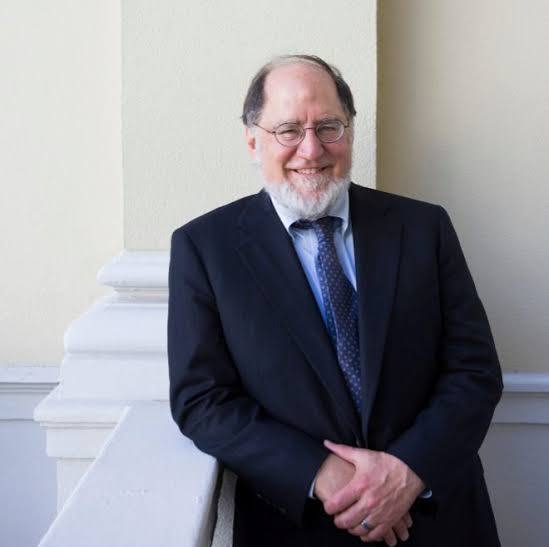
\includegraphics[width=1.0in]{images/rivest.jpeg} & 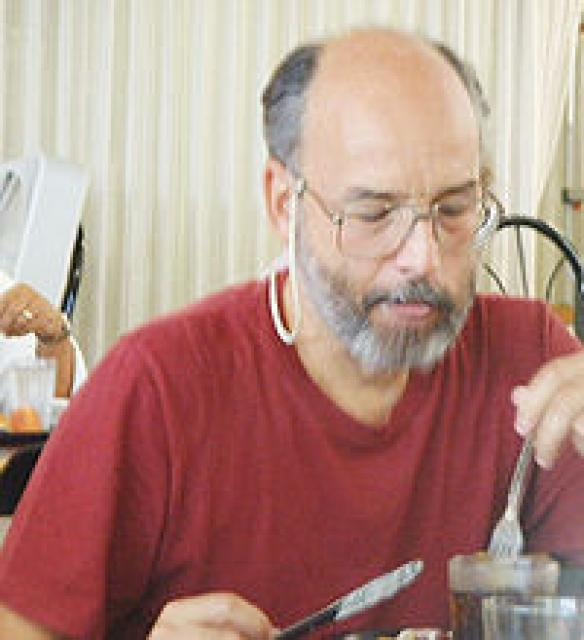
\includegraphics[width=0.9in]{images/adi-shamir-1.jpg} & 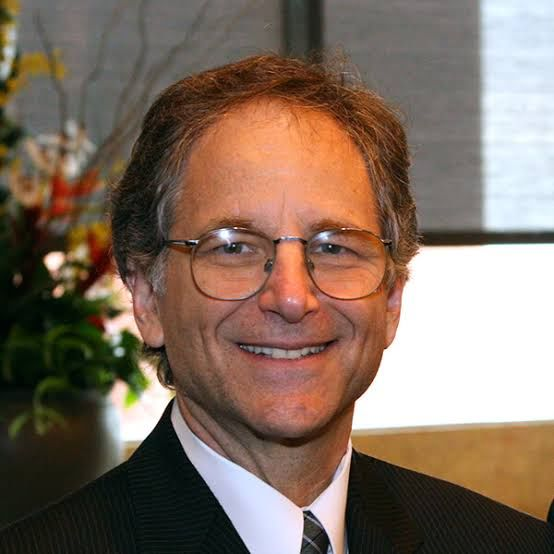
\includegraphics[width=1.0in]{images/adleman.jpeg} \\
Ronald Rivest & Adi Shamir & Leonard Adleman \\
\end{tabular}
\end{center}
\end{figure}
%\begin{figure}[ht]
%\centerline{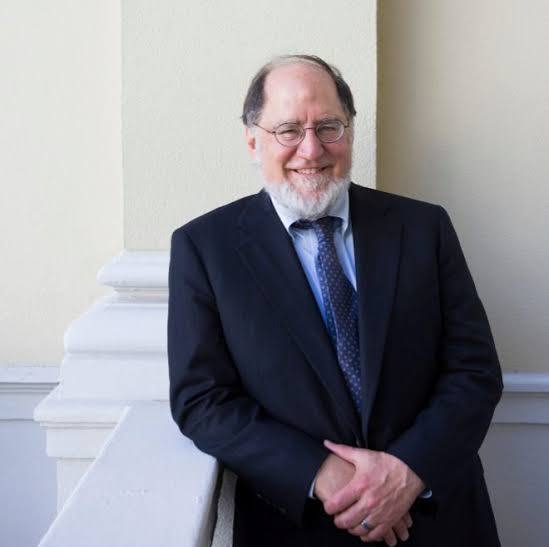
\includegraphics[width=1.0in]{images/rivest.jpeg}}
%\caption*{\small ``We stumbled on public-key cryptography almost by accident, but once we realized what we had, it was like discovering a new continent.'' -- Ron Rivest}
%\end{figure}
%
%\begin{figure}[ht]
%\centerline{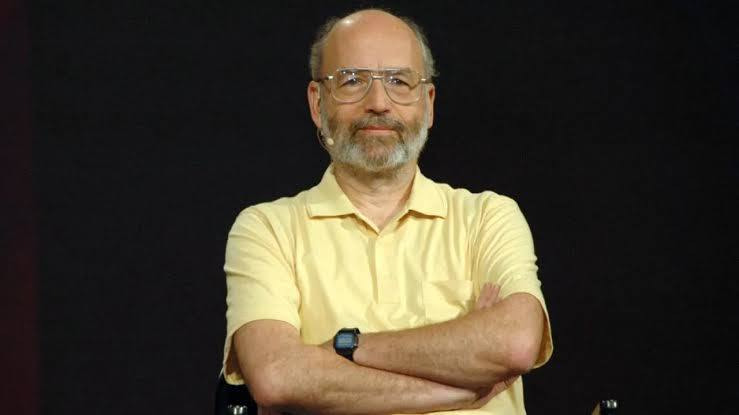
\includegraphics[width=1.0in]{images/shamir.jpeg}}
%\caption*{\small ``Cryptography is the only field where advances in pure mathematics can immediately create or destroy billions of dollars in value.'' -- Adi Shamir}
%\end{figure}
%
%\begin{figure}[ht]
%\centerline{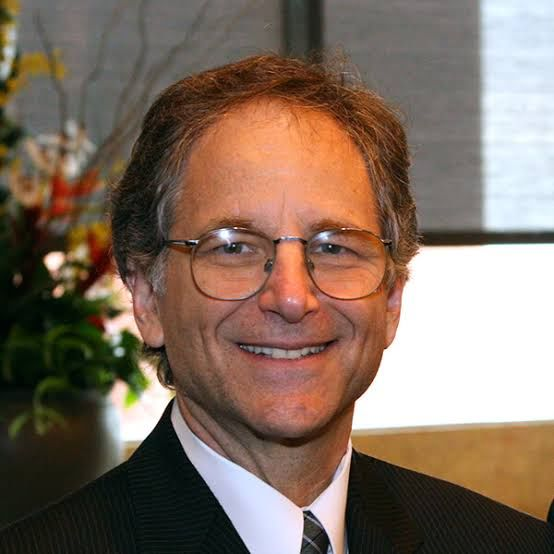
\includegraphics[width=1.0in]{images/adleman.jpeg}}
%\caption*{\small ``RSA worked because of a mathematical truth, not because anyone promised it would.'' -- Leonard Adleman}
%\end{figure}

The \href{https://en.wikipedia.org/wiki/RSA\_cryptosystem}{RSA cryptosystem} was proposed by \href{https://en.wikipedia.org/wiki/Ron\_Rivest}{Ronald Rivest}, \href{https://en.wikipedia.org/wiki/Adi\_Shamir}{Adi Shamir} and
\href{https://en.wikipedia.org/wiki/Leonard\_Adleman}{Leonard Adleman} in 1977. They got the \href{https://en.wikipedia.org/wiki/Turing\_Award}{Turing award} for their result in 2002.

\subsection{The RSA procedure}

To create his public and secret keys, a person uses the following procedure:

\begin{itemize}
\item Select two large prime numbers, $p$ and $q$, typically of 300 to 600 digits each. To select primes, choose random numbers of this size and test for primality using the Fermat's Little Theorem (Theorem \ref{thm:fermat}). By the Prime Number Theorem (Theorem \ref{thm:primenumber}) we are guaranteed to succeed in just a few trials.
\item Compute $n = pq$.
\item Select a small odd integer $e$ that is relatively prime to $m = (p-1)(q-1)$. Use Euclid's GCD to test whether a randomly chosen $e$ is relatively prime to $m$.
\item Compute $d$, the multiplicative inverse of $e$ modulo $m$.  Use the Extended Euclid Algorithm.
\item Publish the pair $P = (e,n)$ as his RSA public key.
\item Keep secret the pair $S = (d,n)$ as his RSA secret key.
\end{itemize}

For this scheme, the domain ${\cal D}$ is $\Z_n = \{0,1,\ldots,n-1\}$. That is,
the message $M$ must be such that $M \in  \Z_n$.The transformation of a message $M$ associated with a public key $P = (e,n)$ is \\
\[
P(M) = M^e \mod n
\]
The transformation of the ciphertext $C$ associated with a secret ket $S = (d,n)$ is \\
\[
S(C) = C^d \mod n
\]

These equations apply both to encryption and signatures.

\subsection{Why does it work?}
It is easy to see  that $P$ and $S$ are inverses:
\[
M^{ed} \equiv M \mod n
\]
\begin{proof}
Note that $m = (p-1)(q-1)$. Since $e$ and $d$ are multiplicative
inverses modulo $m$. We have that
\[
ed = 1 + km = 1 + k(p-1)(q-1)
\]
Thus if $M \not\equiv 0 \mod p$, we have that
\[
\begin{array}{lll}
M^{ed}  & \equiv & M(M^{p-1})^{k(q-1)} \mod p \\
        & \equiv & M(1)^{k(q-1)} \mod p  \\
        & \equiv & M \mod p 
\end{array}
\]
Note that $M^{p-1} \equiv 1 \mod p$ by Fermat's little theorem (Theorem \ref{thm:fermat}).

If $M \equiv 0 \mod p$, we anyway have that
\[
M^{ed} \equiv M \mod p
\]
Repeating the same argument as above, we have that
\[
M^{ed} \equiv M \mod q
\]
Hence, by the Chinese Remainder Theorem (Therem \ref{thm:chinese}) we have that
\[
M^{ed} \equiv M \mod pq \equiv M \mod n
\]
\end{proof}

\subsection{How secure is RSA?}

Multiplying two large primes to form $n$ is easy, but given only $n$ it is extremely difficult to recover $p$ and $q$ with current knowledge.  
RSA security relies on this asymmetry: the public modulus $n$ reveals nothing practical about the private key.  
At present, the only known way to obtain $d$ from $e$ and $n$ is to factor $n$ into its prime factors $p$ and $q$, then compute $m$ and proceed as
above. But no one knows how to factor large integers efficiently, despite several centuries of effort. Using known methods, factoring $n = pq$ where $p$
and q are 600-digit primes would require years on today's fastest supercomputers. Until someone comes up with an efficient way to factor, or discovers some
other way to compute $d$ from $e$ and $n$, the system is reasonably secure for all practical purposes.

RSA remains one of the most commonly use public-key encryption system in the digital world, including in banking, stock markets and other financial trasactions.


\section*{Summary}
\begin{itemize}
\item Primes are the building blocks of integers.
\item Euclid’s algorithm computes gcds efficiently.
\item There are infinitely many primes, and every integer has a unique prime factorisation.
\item Fermat’s little theorem and the CRT are central in modular arithmetic.
\item Public-key cryptography allows secure communication without prior key sharing.
\item RSA uses primes and modular arithmetic, with security based on the difficulty of factoring.
\end{itemize}

\section*{Problems}

\begin{enumerate}

\item \textbf{Prime numbers and factorisation}
  \begin{enumerate}
    \item Prove that there are infinitely many primes of the form $4k+3$.
    \item Factor $123456$ into primes using successive gcd computations.
    \item Use the sieve of Eratosthenes to list all primes up to $200$. 
          How efficient is this compared to trial division?
  \end{enumerate}

\item \textbf{Greatest common divisor}
  \begin{enumerate}
    \item Compute $\gcd(414,662)$ using Euclid’s algorithm. Show all intermediate steps.
    \item Use the extended Euclidean algorithm to find integers $x,y$ such that 
          $414x + 662y = \gcd(414,662)$.
  \end{enumerate}

\item \textbf{Fermat’s little theorem}
  \begin{enumerate}
    \item Verify Fermat’s little theorem for $a=7, p=13$.
    \item Show by counterexample that Fermat’s little theorem does not hold if $p$ is composite.
    \item Explain how Fermat’s little theorem can be used as a primality test. 
          What are its limitations?
  \end{enumerate}

\item \textbf{Chinese remainder theorem}
  \begin{enumerate}
    \item Solve the system of congruences:
      \[
        x \equiv 2 \pmod{3}, \quad 
        x \equiv 3 \pmod{5}, \quad 
        x \equiv 2 \pmod{7}.
      \]
      What is the smallest positive solution?
    \item A recent visitor to Ashoka University, Prof Amartya Kumar Dutta of ISI Kolkata gave the following problems:  
    \begin{enumerate}
    \item In a science camp of 210 students, creativity tests were planned in each of the subjects Mathematics, Physics and Chemistry. The students were to attempt the questions in groups of 5, 6 and 7 respectively. Unfortunately, a few students could not turn up due to unforeseen circumstances and it was found that dividing students into groups of 5, 6 and 7 would leave remainders 2, 1 and 5 respectively. Using ku\d{t}\d{t}aka, a professor of mathematics quickly realised how many students were present and suggested how the students could be grouped if uniformity in number was to be insisted. What was the total number of students present?
    \item (Hardy-Wright) From Monday, 1 January 2018, six professors begin two-year courses of lectures on Monday, Tuesday, Wednesday, Thursday, Friday, and Saturday. They announce their intention of lecturing at intervals of two, three, four, one, six, and five days respectively. However, no lecture is to take place on a Sunday and a professor would omit his lecture if it falls on a Sunday. For instance, the dates of the lectures of the first professor were January 1,3,5,9,11,13, … (omitting 7 January, a Sunday). What will be the date of the first Sunday on which all six professors find themselves compelled to omit a lecture?
    \end{enumerate}
    \item Explain why the Chinese Remainder Theorem is crucial for speeding up RSA decryption.
  \end{enumerate}

\item \textbf{Cryptography and RSA}
  \begin{enumerate}
    \item Work out a small RSA example: choose primes $p=17, q=23$, construct public/private keys, 
          and encrypt/decrypt the message $M=42$.
    \item Suppose Eve can factor the modulus $n$. Show why RSA becomes insecure.
    \item Consider the Caesar cipher. Implement it with shift $k=3$, encrypt the message ``HELLO'', 
          then decrypt it.
    \item Compare the Caesar cipher with RSA in terms of key space, security, and vulnerability to 
          brute-force attack.
  \end{enumerate}

\item \textbf{Reflection and open-ended problems}
  \begin{enumerate}
    \item Discuss why factoring large numbers is computationally difficult, and why this difficulty 
          underpins public-key cryptography.
    \item Research the Miller--Rabin primality test. How does it improve upon Fermat’s test?
    \item Find a real-world application where digital signatures are used. 
          Explain the role of public and private keys in that context.
  \end{enumerate}

\end{enumerate}
